\subsection{\ac{rltanlage} Vergangenheit}
Lüftungsgeräte sind schon seit längerer Zeit in Verwendung \zB in Wirtschaftsbetrieben, Gastronomie aber auch in Bürogebäuden. Die Ursprünge von Lüftungsgeräten bzw. \ac{rltanlage} lassen sich jedoch schon auf ca. 3000 v. Chr. datieren.
Die ersten Versuche fanden dahingehen Anwendung, um Höhlen und Unterkünfte vom Rauch des Feuers zu befreien. Es wurden solche Arten von Raumbelüftungen \zB in Ondol in Alaska gefunden.
Lüftungstechnik wurde damals durch den natürlichen Wetterzyklus bestimmt. 
Erst im späteren Verlauf wurde, durch die Entwicklung moderner Belüftungs- und Klimatechnik, die aktive Belüftung- und Temperaturregelung möglich.

Die ersten Gehversuche einer richtigen \acs{rltanlage} wurde 1836 im House of Commons in London gemacht. Die Anlage umfasst alle Punkte einer \acs{rltanlage}: Heizen, Kühlen, Be- und Entfeuchten sowie Filtern der Luft. 

Die folgende Beschreibung bezieht sich auf
Abb.~\ref{fig:House_of_Commons_Klimatechnik}.
Die Anlage versorgte das House of Commons mit Zuluft welche links unten bei den Gitter angesaugt wird (Die Ansaugung der Frischluft lag knapp über der Themse). Die Kühlung wurde durch Eis welches in der Kammer hinter den Gittern liegt realisiert.
Die Filterung wurde durch Baumwolle, welche bei Punkt C aufgeschichtet wird realisiert.
Nach der Filterung wurde beim Punkt A die Luft erhitzt. 
Danach strömte die Luft durch den doppelten Boden und wurde dadurch verteilt. Die Luft strömte nun nach oben und wurde bei Punkt F aus dem Gebäude geleitet. Im Winter leitete man die Luft nach links direkt aus dem Fenster geleitet. Im Sommer hingegen wurde die Luft nach rechts durch die Verrohung und durch den Kamin  nach draußen geleitet. vgl.
\cite[vgl.][]{Fitzner_Finke:2010} 

\begin{figure}[ht]
	\centering
	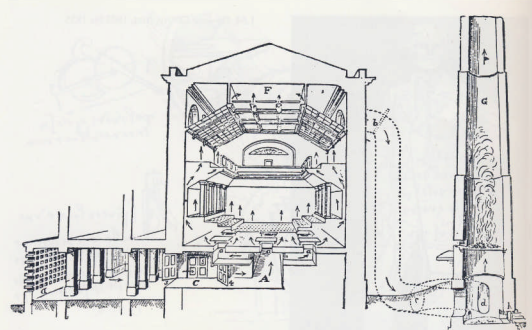
\includegraphics[width=0.6\linewidth]{Bilder/Belueftung_House_of_Commons}
	\caption{Klimatechnik House of Commons  (Quelle: \url{https://vhkk.org/page/vortrag/pdf/Geschichte_Raumklimatechnik.pdf})}
	\label{fig:House_of_Commons_Klimatechnik}
\end{figure}



\subsection{\ac{rltanlage} Gegenwart}
Die Funktionen einer \ac{rltanlage} unterscheiden sich grundsätzlich nicht wirklich von dem was schon z.B. 1836 im House of Commons in London verwendet wurde. Die einzelnen Abschnitte wie \zB Ansaugung, Filtration, Be- und Entfeuchtung, Kühlung, Heizung und Absaugung haben sich, in deren Funktionen (Zweck), wenig verändert. Der Aufbau, die Funktionsweise und die Umsetzung der einzelnen Abschnitte änderte sich  grundlegend.

Der Aufbau hat sich dahingehend restrukturiert, dass eine moderne \ac{rltanlage} sehr kompakt im Aufbau ist. Angefangen bei den Steuerungsklappen für Zu- bzw. Abluft über die Ventilatoren, das Heiz- bzw. Kühlregister, die Wärmetauscher, die Filter und der Luft Be- und Entfeuchter, ist alles in einer \ac{rltanlage} untergebracht.
Die \ac{rltanlage} wird von außen mit leichten Aluminiumplatten verkleidet, welche von innen Schall- und Wärme-isoliert sind. Dies ist dahingehend wichtig, da die \acp{rltanlage} meist außerhalb, \zB auf Dächern oder hinter dem Haus angeschlossen/installiert werden. 

Im folgenden werden die Komponenten anhand des allgemeinen Aufbauplans einer \ac{rltanlage} Abb.~\ref{fig:Aufbau_Lueftungsgerät_allgemein} beschrieben. 

\begin{figure}[H]
	\centering
	\includegraphics[width=0.9\linewidth]{Bilder/Lueftungsgerät_allgemein_aufbau}
	\caption{Allgemeiner Aufbau einer \ac{rltanlage} (Quelle: \url{https://www.baunetzwissen.de/gebaeudetechnik/fachwissen/lueftung/bestandteile-von-lueftungsanlagen-2473103})}
	\label{fig:Aufbau_Lueftungsgerät_allgemein}
\end{figure}

\subsection{\ac{rltanlage} allgemein}
\begin{itemize}
	\item \textbf{Ventilatoren}: In einer \ac{rltanlage} ist immer mindestens ein Ventilator vorhanden (abhängig der Größe der \ac{rltanlage}). Dieser ist für die Beförderung von Luftmassen durch die \ac{rltanlage} sowie die Beförderung aus und in das Gebäude zuständig. Der Ventilator muss mit Bedacht dimensioniert sein, da dieser in der \ac{rltanlage} den höchsten Stromverbrauch hat. Die Dimensionierung muss so gewählt werden, dass der intern herrschende Strömungswiderstand überwindet wird. Es gibt verschiedene Arten von Ventilatoren 
\begin{itemize}
	\item Axialventilatoren mit/ohne Leitrad Abb.~\ref{fig:EBM_Axialventilator}
	\item Radialventilatoren mit Laufräder (vorwärts- oder rückwertsgekrümmte Schaufeln)
	\item Querstrom- oder Tangentiallüfter 
\end{itemize}

\begin{figure}[H]
	\centering
	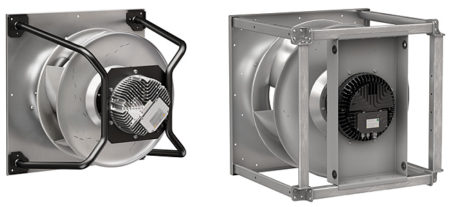
\includegraphics[width=0.5\linewidth]{Bilder/axialventilator}
	\caption{EBM Axialventilator} 
	(Quelle: \url{https://ebmpapst-7237.kxcdn.com/de/files/2017/11/RadiPac-mit-oder-ohne-tragspinne-450x207.jpg})
	\label{fig:EBM_Axialventilator}
\end{figure}

	\item \textbf{Heiz- und Kühlregister}: im Heiz- und Kühlregister Abb.~\ref{fig:heizregister} wird die einströmende Luft je nach Bedürfnis erhitzt oder gekühlt. Dies wird durch unterschiedlichste Heiz- oder Kühlmedien realisiert bsp. Dampf, heißes oder kaltes Wasser, welches durch das Heiz- bzw. Kühlregister fließt. Andere Arten um die einströmende Luft zu erhitzen sind: Elektrolufterhitzer, gasbetriebene Lufterhitzer. Um die Luft abzukühlen kann auch ein Direktverdampfer verwendet werden.
	Um Energiekosten zu sparen, wird der Abluft die Wärmeenergie entzogen und der Zuluft wieder hinzugefügt, dabei werden bis zu 98 Prozent der Wärmeenergie zurückgewonnen. Im Vergleich zu \ac{rltanlage} ohne Wärmerückgewinnung werden bis zu 30 Prozent an Heizenergie eingespart. 

\begin{figure}[H]
	\centering
	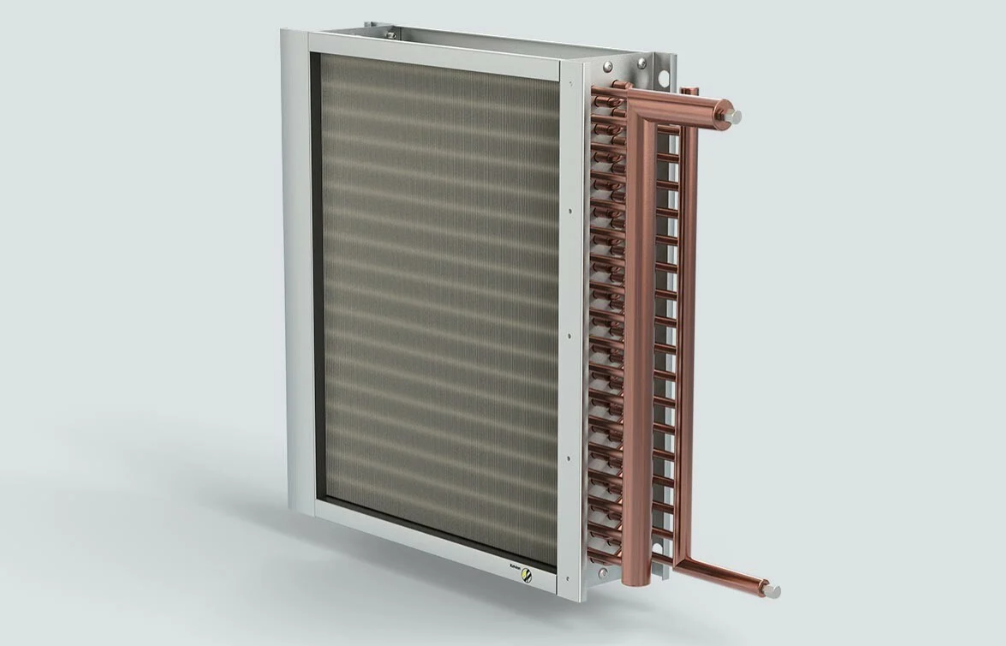
\includegraphics[width=0.5\linewidth]{Bilder/luftwaermeregister}
	\caption{Heiz- Kühlregister} 
	(Quelle: \url{https://www.baunetzwissen.de/gebaeudetechnik/fachwissen/lueftung/bestandteile-von-lueftungsanlagen-2473103/gallery-1/5})
	\label{fig:heizregister}
\end{figure}

	\item \textbf{Luft Be- und Entfeuchter}: Der Luft Be- und Entfeuchter Abb.~\ref{fig:luftbefeuchter} ist dafür zuständig, dass die Zuluft und dessen Luftfeuchtigkeit den Sollwert nicht unter- bzw. überschreiten. Meist wird für diesen Schritt ein Umlaufsprühbefeuchter eingesetzt. Dieses Bauteil ist jedoch zwecks dessen Hygiene, sehr Wartungsintensiv. 

\begin{figure}[H]
	\centering
	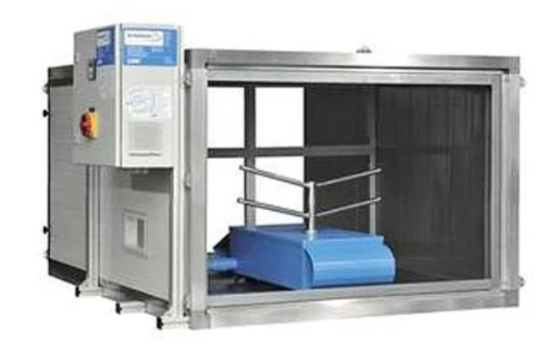
\includegraphics[width=0.5\linewidth]{Bilder/Luftbefeuchter}
	\caption{Luftbe- und Entfeuchter} 
	(Quelle: \url{	https://www.baunetzwissen.de/gebaeudetechnik/fachwissen/lueftung/bestandteile-von-lueftungsanlagen-2473103/gallery-1/6})
	\label{fig:luftbefeuchter}
\end{figure}

\item \textbf{Filter}: Die verbauten Filter sind für die Filterung der Zuluft zuständig. Filter werden laut der DIN EN ISO 16890-1 in 3 Gruppen unterteilt.
\begin{itemize}
	\item PM(Particulate Matter) 1: Partikel die größer als 1 Mikrometer sind \zB Viren oder Verbrennungspartikel 
	\item PM(Particulate Matter) 2,5: Partikel die größer als 2,5 Mikrometer sind \zB Bakterien oder Pilze
	\item PM(Particulate Matter) 10: Partikel die größer als 10 Mikrometer sind \zB Pollen oder Staub
\end{itemize}
Es werden zur Reinigung der Zuluft entweder Taschenfilter Abb.~\ref{fig:taschenfilter} oder Kassettenfilter verwendet. Um Gerüche aus der Luft zu filtern \zB in Küchen werden Aktivkohlefilter verwendet. Bei beiden Filterarten ist es wichtig diese in regelmäßigen Abständen zu säubern oder ersetzten.  

\begin{figure}[H]
	\centering
	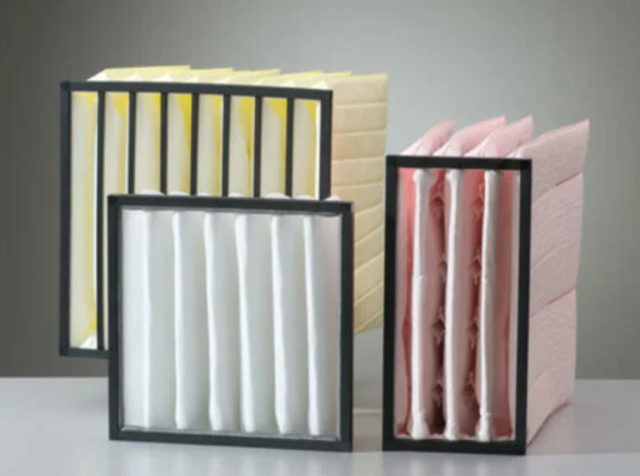
\includegraphics[width=0.5\linewidth]{Bilder/normalefilter}
	\caption{Taschenfilter} 
	(Quelle: \url{	https://www.baunetzwissen.de/gebaeudetechnik/fachwissen/lueftung/bestandteile-von-lueftungsanlagen-2473103/gallery-1/7})
	\label{fig:taschenfilter}
\end{figure}

	\item \textbf{Schalldämpfer}: Schalldämpfer Abb.~\ref{fig:schalldaempfer} sind für die Absorption von Lärmquellen in einem Lüftungsgerät zuständig. Die Lärmquelle mit dem höchsten Lärmpegel sind dabei die Ventilatoren. Es wird dabei unterschieden zwischen:
\begin{itemize}
	\item Absorptions-Schalldämpfer 
	\item Drossel-Schalldämpfer
	\item Resonanz-Schalldämpfer
\end{itemize} 
	Auch die richtige Anordnung und Dimensionierung der Verrohung zwischen einzelnen Räumen, welche an der selben \ac{rltanlage} angeschlossen sind ist essenziell. Dabei werden Strömungsgeräusche (Geräusch welche zwischen zwei Räumen durch die Verrohung transportiert werden) verhindern.

\begin{figure}[H]
	\centering
	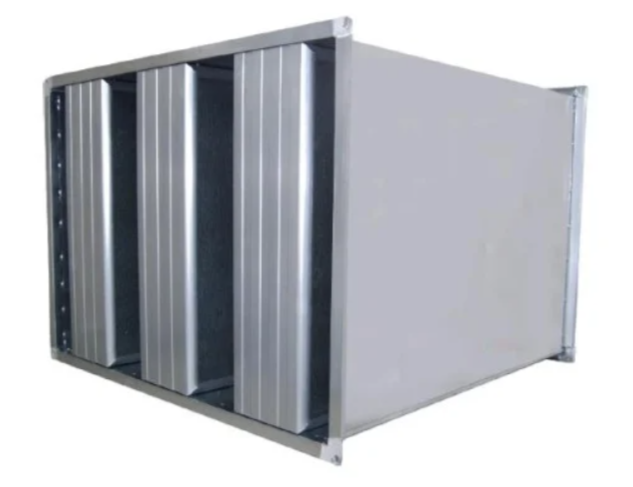
\includegraphics[width=0.5\linewidth]{Bilder/schalldaempfer}
	\caption{Schalldämpfer (Mineralwolle als Dämpfmaterial)} 
	(Quelle: \url{	https://www.baunetzwissen.de/gebaeudetechnik/fachwissen/lueftung/bestandteile-von-lueftungsanlagen-2473103/gallery-1/8})
	\label{fig:schalldaempfer}
\end{figure}

	\item \textbf{Drossel- und Jalousieklappen}: 
	Drossel- und Jalousieklappen Abb.~\ref{fig:drosselklappe} werden dahingehend eingesetzt, um durchgehend einen konstanten Volumenstromwert zu erreichen. 

\begin{figure}[H]
	\centering
	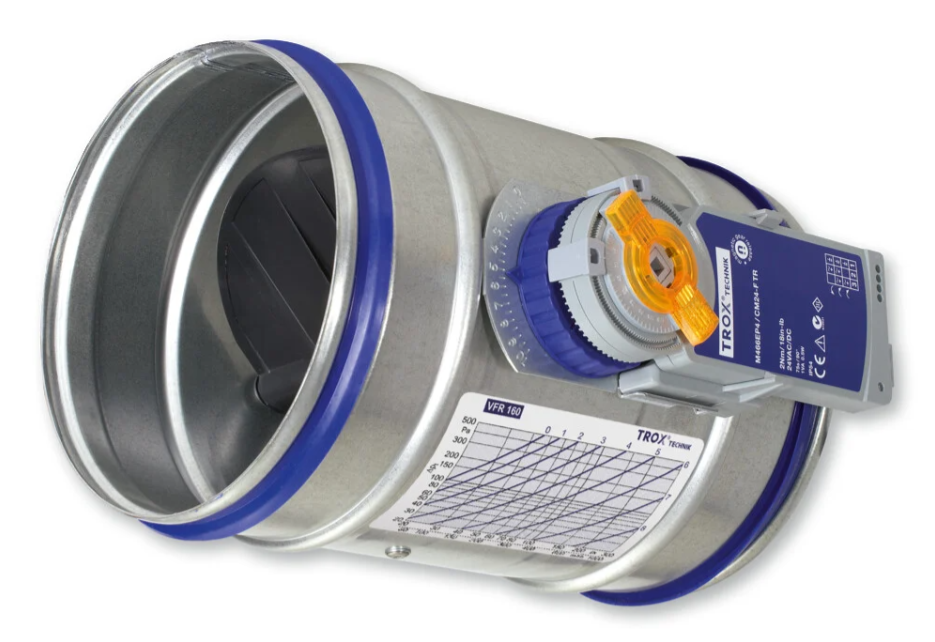
\includegraphics[width=0.5\linewidth]{Bilder/drosselklappe}
	\caption{Drosselklappe} 
	(Quelle: \url{	https://www.baunetzwissen.de/gebaeudetechnik/fachwissen/lueftung/bestandteile-von-lueftungsanlagen-2473103/gallery-1/10})
	\label{fig:drosselklappe}
\end{figure}

	\item \textbf{Volumenstromregler}: Der Volumenstromregler arbeitet eng mit den Drossel- und Jalousieklappen zusammen. Dabei wird zwischen einem Konstant-Volumenstromregler oder einem variablen Volumenstromregler. Wie aus dem Namen abzuleiten, ist dieser für die Messung und Regelung des Luftvolumens zuständig. 

\begin{figure}[H]
	\centering
	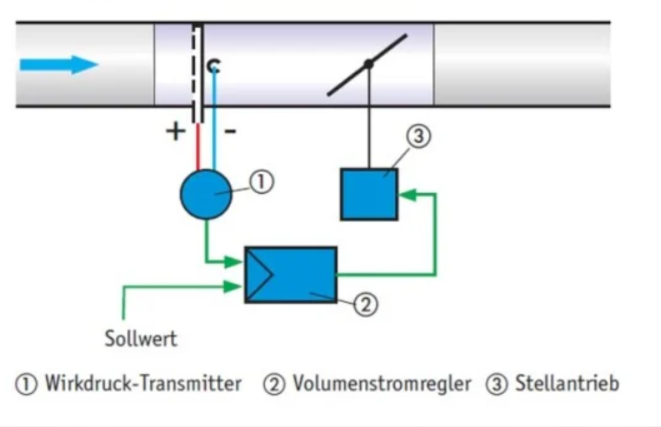
\includegraphics[width=0.5\linewidth]{Bilder/volumenstromregler}
	\caption{Volumenstromregler} 
	(Quelle: \url{	https://www.baunetzwissen.de/gebaeudetechnik/fachwissen/lueftung/bestandteile-von-lueftungsanlagen-2473103/gallery-1/12})
	\label{fig:volumenstromregler}
\end{figure}

	\item \textbf{Brandschutzklappen und Rauchschutzklappen}:
	Die Sicherheit vor Feuer und Rauch ist durch sogenannte Brand- und Rauchschutzklappen gegeben.
	Diese Art von Klappen verhindert das sich Rauch oder Feuer über die Lüftungsschächte/Verrohung durch das Gebäude ausbreitet. Brandschutzklappen Abb.~\ref{fig:Brandschutzklappe} sind zwischen den einzelnen Brandabschnitten eines Gebäudes angebracht. Rauchschutzklappen Abb.~\ref{fig:Rauchschutzklappe} sind im inneren der Lüftungsleitungen angebracht, dadurch wird verhindert, dass Menschen giftige Dämpfe und Rauch einatmen. Sowohl die Brandschutzklappe als auch die Rauchschutzklappe, schließen im Notfall (Brand- oder Rauchentwicklung) automatisch.
\end{itemize}

\begin{figure}[H]
	\centering
	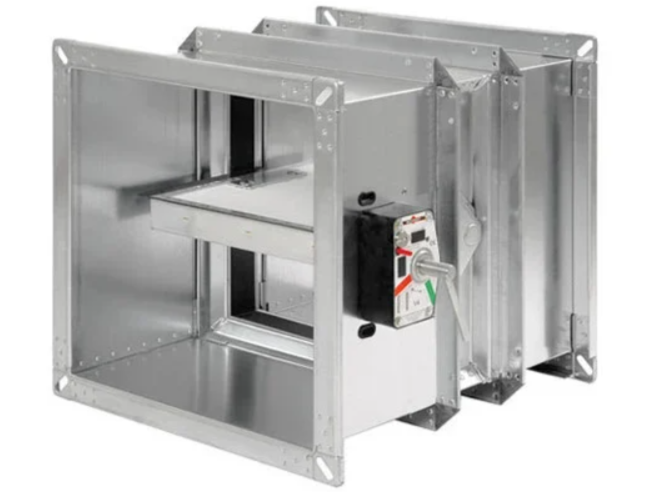
\includegraphics[width=0.5\linewidth]{Bilder/brandschutzklappe}
	\caption{Automatische Brandschutzklappe} 
	(Quelle: \url{	https://www.baunetzwissen.de/gebaeudetechnik/fachwissen/lueftung/bestandteile-von-lueftungsanlagen-2473103/gallery-1/14})
	\label{fig:Brandschutzklappe}
\end{figure}

\begin{figure}[H]
	\centering
	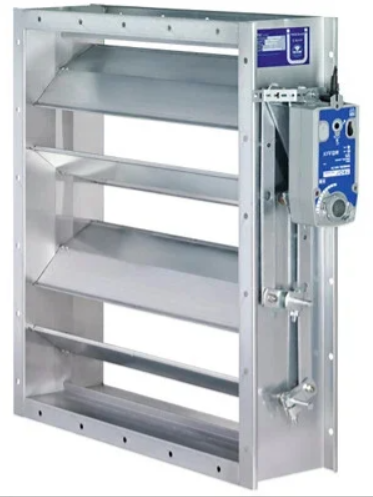
\includegraphics[width=0.5\linewidth]{Bilder/rauchschutzklappe}
	\caption{Rauchschutzklappe} 
	(Quelle: \url{	https://www.baunetzwissen.de/gebaeudetechnik/fachwissen/lueftung/bestandteile-von-lueftungsanlagen-2473103/gallery-1/15})
	\label{fig:Rauchschutzklappe}
\end{figure}

\cite[vgl.][]{baunetz_bestandteile_nodate:o.J.}

\subsection{\ac{rltanlage} Einsatzbereiche / Verwendungszweck}

\ac{rltanlage}n werden dahingehend eingesetzt um in Räumen oder Gebäuden die drei wichtigen Bereich der Raumlufttechnik abzudecken:

\begin{itemize}
	\item Lufttemperatur
	\item Luftfeuchtigkeit
	\item Luftqualität
\end{itemize} 

Dabei fördert die \ac{rltanlage} die verbrauchte Luft nach draußen. Die Luft wird bevor sie in die Umwelt gelassen wird gefiltert. Das ist wichtig, da die Luft welche in Industriebetrieben \zB einer Druckerei abgelassen wird, meist mit Schadstoffen versetzt sind. Diese Schadstoffe müssen abgelassen werden, da diese für den Menschen gesundheitsschädlich sein können. Durch das absaugen von Gefahrenstoffe aus der Luft, erhöht sich die Sicherheit der Mitarbeiter bezüglich der Gesundheit.

Durch die Speisung der frischer Zuluft und Absaugung der verbrauchten Abluft können Schadstoffpartikel, Viren und ein gewisses Maß an zu hoher oder zu niedriger Raumtemperatur und Raumluftfeuchtigkeit ausgeglichen werden. 
\cite[vgl.][]{DGWZ:o.J.}

Neben der vorher genannten Industrie werden \ac{rltanlage}n auch im medizinischen Sektor eingesetzt. In diesem Sektor wird der Fokus verstärkt auf die Luftqualität gelegt. Eine \ac{rltanlage} muss im medizinischen Sektor, zu jeder Zeit die Versorgung über die Zuluft mit frischem Sauerstoff gewährleistet sein. Die Abführung ist auch wichtig um verbrauchte (Kohlendioxyd haltige) Luft aus dem Operationssaal zu leiten. Zusätzlich muss im medizinischen Sektor der angeordnete Schutzbereich (\zB Operationssaal, Reinraum) besonders vor Kontamination geschützt werden. Dies wird meist mit einem leichten Überdruck gewährleistet, dass keine Kontamination (Viren etc.) mit außenliegender, nicht gefilteter Luft besteht.
\cite[vgl.][]{robatherm:2019,robatherm:o.J.}

Weitere Einsatzbereiche sind:
\begin{itemize}
	\item Labore
	\item Bürogebäude, Bildungsstätten (Schulen, Kindergarten)
	\item Küchen (Gastronomie)
	\item Verkaufsstätten
	\item Schwimmbäder
\end{itemize} 
\cite[vgl.][]{robatherm:2019,induux_wiki:2023}

\subsection{\ac{rltanlage} Walter-Bösch GmbH. (tdot-Gerät)}

-funktion (allgemein, Gerät tdot und walter bösch geräte) wichtigkeit. 


